% ============================================================
%  ANNEXURE  — custom title command
%  Mimics the numbered-chapter style: title vertically centred
%  on its own page, content begins on the NEXT page.
% ============================================================
\newcommand{\annexuretitle}[1]{%
  \clearpage
  \thispagestyle{plain}%
  \vspace*{\fill}
  {\centering
    \normalfont\Large\bfseries
    \MakeUppercase{#1}\par
  }%
  \vspace*{\fill}
  \addcontentsline{toc}{chapter}{#1}%
  \clearpage
  \thispagestyle{fancy}%
}

% ── Annexure - A ─────────────────────────────────────────────
\annexuretitle{Annexure - A}

\begin{singlespacing}\small

\section*{API Endpoint Reference}
\vspace{-0.5em}
\begin{table}[H]
\centering
\caption{MindTrace REST API Endpoints}
\renewcommand{\arraystretch}{1.1}
\begin{tabular}{lllp{4.5cm}}
\toprule
\textbf{Method} & \textbf{Endpoint}       & \textbf{Auth} & \textbf{Description} \\
\midrule
POST   & \texttt{/register}          & No    & Register a new user account \\
POST   & \texttt{/login}             & No    & Login and receive JWT token \\
POST   & \texttt{/api/analyze}       & Yes   & Submit webcam frame for analysis \\
POST   & \texttt{/api/session/start} & Yes   & Create a new session record \\
POST   & \texttt{/api/session/end}   & Yes   & Finalise and save current session \\
GET    & \texttt{/api/sessions}      & Yes   & Retrieve current user's sessions \\
GET    & \texttt{/api/admin/users}   & Admin & Retrieve all user records \\
GET    & \texttt{/api/admin/sessions}& Admin & Retrieve all sessions (all users) \\
\bottomrule
\end{tabular}
\end{table}

\vspace{0.3em}
\section*{Sample API Request and Response}
\vspace{-0.3em}
\textbf{Request} — POST \texttt{/api/analyze}:
\vspace{-0.5em}
\begin{verbatim}
{
  "frame": "<base64-encoded JPEG string>",
  "session_id": "6614f3a2c3e4b12a9d7f0011"
}
\end{verbatim}
\vspace{-1em}
\textbf{Response}:
\vspace{-0.5em}
\begin{verbatim}
{
  "emotion": "Happy",
  "confidence": 0.91,
  "engagement_score": 87,
  "head_pose": {
    "pitch": -2.3,
    "yaw":    4.1,
    "roll":   1.8
  },
  "blink_rate": 14
}
\end{verbatim}

\end{singlespacing}

% ── Annexure - B ─────────────────────────────────────────────
\annexuretitle{Annexure - B}

\section*{Technology Stack Summary}

\begin{table}[H]
\centering
\caption{Complete Technology Stack}
\begin{tabular}{lll}
\toprule
\textbf{Layer}        & \textbf{Technology}         & \textbf{Version} \\
\midrule
ML Framework          & PyTorch + torchvision       & 2.x \\
Model Architecture    & ResNet-18 (fine-tuned)      & --- \\
Face Detection        & MediaPipe Face Mesh         & 0.10+ \\
Computer Vision       & OpenCV                      & 4.x \\
API Framework         & FastAPI + Uvicorn           & 0.110+ \\
Database              & MongoDB Atlas + Motor       & 6.x \\
Authentication        & PyJWT + bcrypt              & --- \\
Frontend Framework    & React + Vite                & 18.x / 5.x \\
Charting Library      & Recharts                    & 2.x \\
HTTP Client           & Axios                       & 1.x \\
Backend Deployment    & Hugging Face Spaces (Docker)& --- \\
Frontend Deployment   & Vercel                      & --- \\
Version Control       & Git + GitHub                & --- \\
\bottomrule
\end{tabular}
\end{table}

\section*{Emotion Score Weights}

The engagement score is computed using the following empirically determined
weights applied to the three signal components:

\begin{table}[H]
\centering
\caption{Engagement Score Component Weights}
\begin{tabular}{lcc}
\toprule
\textbf{Component}     & \textbf{Weight} & \textbf{Rationale} \\
\midrule
Emotion score ($S_e$)  & 0.50            & Primary indicator of cognitive state \\
Head pose score ($S_p$)& 0.35            & Strong proxy for visual attention \\
Blink rate score ($S_b$)& 0.15          & Supplementary fatigue indicator \\
\midrule
\textbf{Total}         & \textbf{1.00}   & --- \\
\bottomrule
\end{tabular}
\end{table}

% ── Annexure - C ─────────────────────────────────────────────
\annexuretitle{Annexure - C}

\section*{Plagiarism Report}

The following pages contain the plagiarism check report generated for this
project document, confirming the originality of the submitted work.

\vspace{0.5em}

\begin{figure}[H]
  \centering
  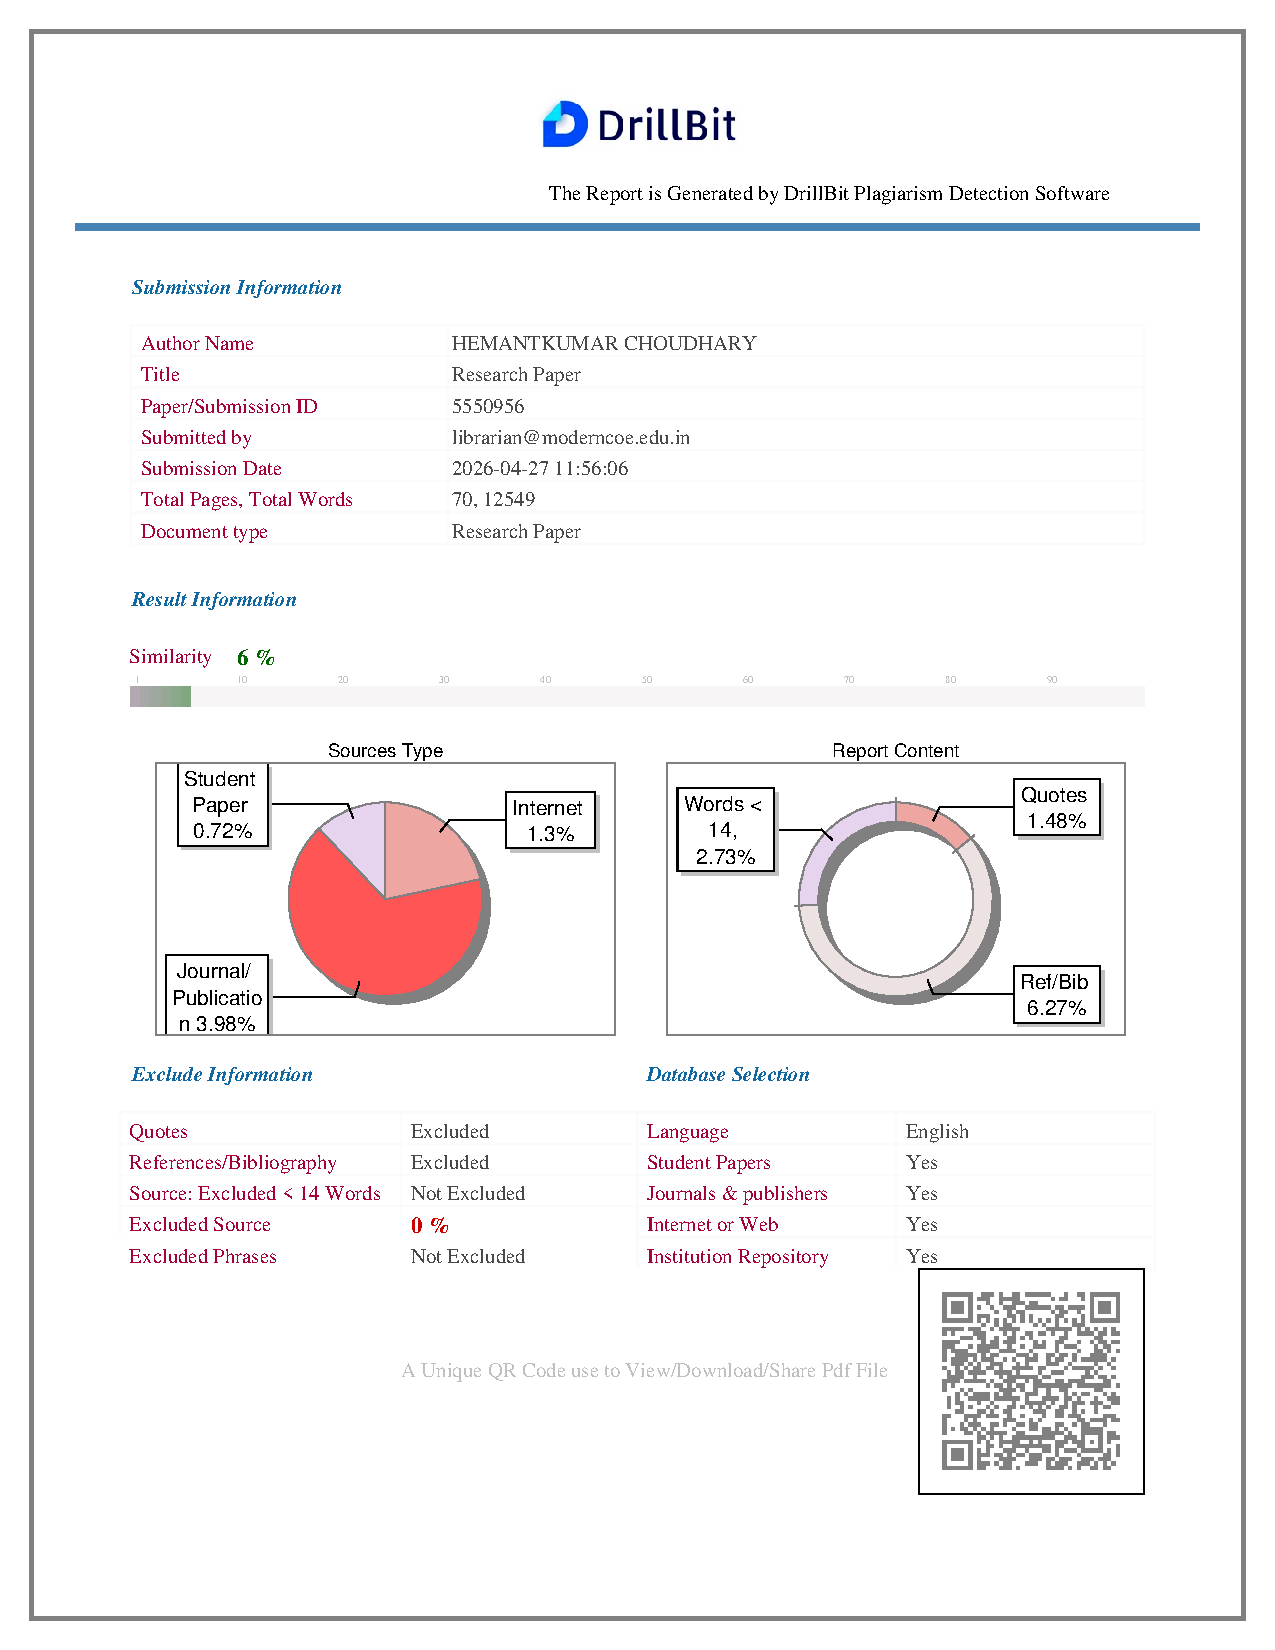
\includegraphics[page=1,width=0.85\linewidth,keepaspectratio]{Plagiarism Report 1.pdf}
  \caption[]{Plagiarism Report Page 1}% suppress auto LOF entry
\end{figure}
\addcontentsline{lof}{figure}{Plagiarism Report Page 1}% manual unnumbered LOF entry

\newpage
\begin{figure}[H]
  \centering
  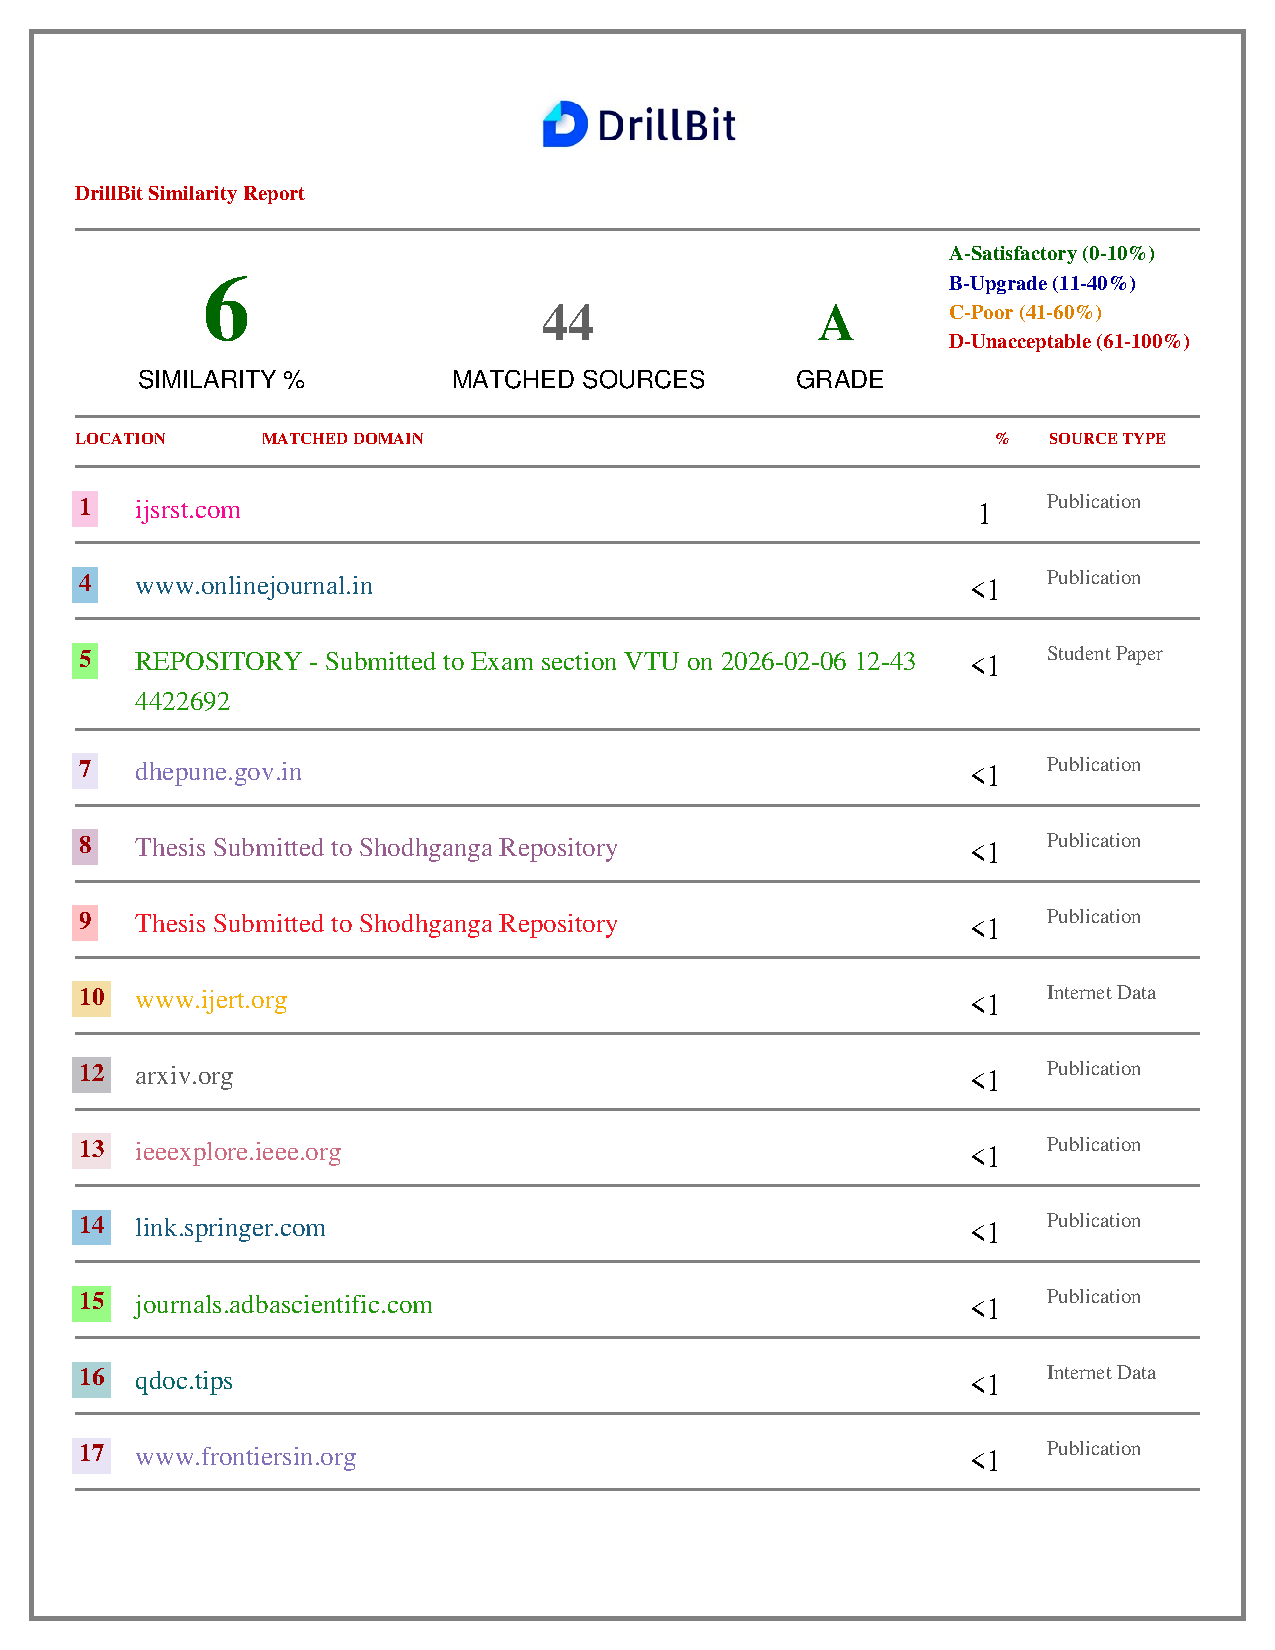
\includegraphics[page=1,width=0.85\linewidth,keepaspectratio]{Plagiarism Report 2.pdf}
  \caption[]{Plagiarism Report Page 2}% suppress auto LOF entry
\end{figure}
\addcontentsline{lof}{figure}{Plagiarism Report Page 2}% manual unnumbered LOF entry
